\documentclass[border=6pt]{standalone}
% Shared preamble for web figures.  Each figure is a standalone .tex that
% \input's this file; scripts/make-figures.sh turns it into an SVG.
% Handouts pull the same file with \fig{Unit_X/<name>}.
\usepackage[T1]{fontenc}
\usepackage{helvet}
\renewcommand{\familydefault}{\sfdefault}
\renewcommand{\ttdefault}{pcr}  % Courier: a real Type 1 typewriter font
\usepackage{amsmath}
\usepackage{tikz}
\usetikzlibrary{arrows.meta,positioning,calc,shapes.symbols,shapes.geometric}

% Who makes the rules is the point of most diagrams in this book, so the
% colors mean the same thing everywhere: blue is a person, orange is the
% computer, green is an answer, pink is the human brain.
\definecolor{person}{HTML}{2C6FAE}
\definecolor{machine}{HTML}{D35400}
\definecolor{result}{HTML}{1E8449}
\definecolor{brainpink}{HTML}{C2185B}
\definecolor{ink}{HTML}{2C3E50}

\tikzset{
  doodle/.style={line width=1.5pt, line cap=round, line join=round, draw=ink},
  box/.style={draw, rounded corners=5pt, line width=1.1pt, align=center,
              inner sep=7pt, minimum height=1.0cm, font=\small},
  personbox/.style={box, draw=person, fill=person!10},
  machinebox/.style={box, draw=machine, fill=machine!10},
  resultbox/.style={box, draw=result, fill=result!10},
  plainbox/.style={box, draw=ink!70, fill=ink!4},
  flow/.style={-{Stealth[length=8pt]}, line width=1.4pt, draw=ink},
}

% A person (blue) and a robot head (orange) as small icons.
% \personicon{x}{y}{scale}   \roboticon{x}{y}{scale}
\newcommand{\personicon}[3]{%
  \begin{scope}[shift={(#1,#2)}, scale=#3]
    \fill[person] (0,0.62) circle (0.28);
    \fill[person, rounded corners=6pt] (-0.42,-0.55) rectangle (0.42,0.28);
  \end{scope}}
\newcommand{\roboticon}[3]{%
  \begin{scope}[shift={(#1,#2)}, scale=#3]
    \draw[machine, line width=1.2pt] (0,0.5) -- (0,0.72);
    \fill[machine] (0,0.78) circle (0.08);
    \draw[machine, line width=1.4pt, fill=machine!12, rounded corners=4pt] (-0.5,-0.45) rectangle (0.5,0.5);
    \fill[ink] (-0.2,0.12) circle (0.08);
    \fill[ink] (0.2,0.12) circle (0.08);
    \draw[ink, line width=1pt] (-0.22,-0.22) -- (0.22,-0.22);
  \end{scope}}

\begin{document}
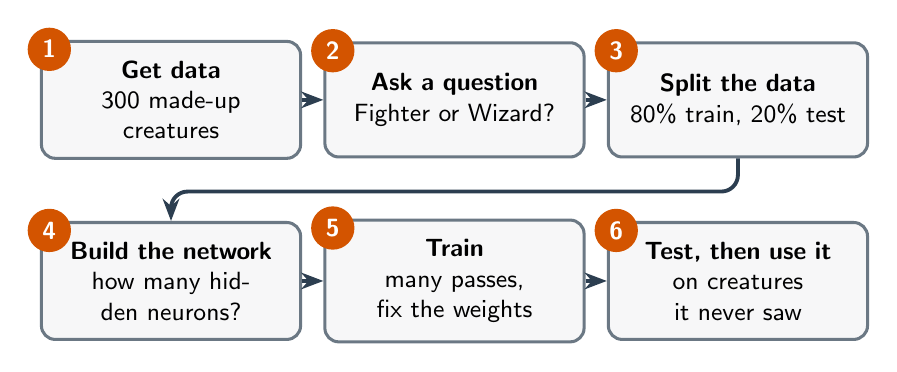
\begin{tikzpicture}[
  st/.style={plainbox, minimum width=3.0cm, minimum height=1.45cm, text width=2.8cm, font=\small},
  num/.style={circle, fill=machine, text=white, font=\bfseries\small, inner sep=1.5pt, minimum size=0.55cm},
]
% How to build an AI, in the order the 2.6 tool does it.
\foreach \i/\x/\y/\t in {1/0/0/{\textbf{Get data}\\300 made-up creatures}, 2/3.6/0/{\textbf{Ask a question}\\Fighter or Wizard?}, 3/7.2/0/{\textbf{Split the data}\\80\% train, 20\% test},
                        4/0/-2.3/{\textbf{Build the network}\\how many hidden neurons?}, 5/3.6/-2.3/{\textbf{Train}\\many passes, fix the weights}, 6/7.2/-2.3/{\textbf{Test, then use it}\\on creatures it never saw}} {
  \node[st] (s\i) at (\x,\y) {\t};
  \node[num] at ($(s\i.north west)+(0.12,-0.12)$) {\i};
}
\draw[flow] (s1) -- (s2); \draw[flow] (s2) -- (s3);
\draw[flow, rounded corners=6pt] (s3.south) -- ($(s3.south)+(0,-0.42)$) -| (s4.north);
\draw[flow] (s4) -- (s5); \draw[flow] (s5) -- (s6);
\end{tikzpicture}
\end{document}
